
%--------------------------------------------------------------------
%--------------------------------------------------------------------
% Formato para los talleres del curso de Métodos Computacionales
% Universidad de los Andes
% 2015-10
%--------------------------------------------------------------------
%--------------------------------------------------------------------

\documentclass[11pt,letterpaper]{exam}
\usepackage[utf8]{inputenc}
\usepackage[spanish]{babel}
\usepackage{graphicx}
\usepackage{mdframed}
\usepackage{tabularx}
\usepackage[absolute]{textpos} % Para poner una imagen completa en la portada
\usepackage{multirow}
\mdfdefinestyle{mystyle}{leftmargin=1cm,rightmargin=1cm,linecolor=red}
\usepackage{float}
\usepackage{hyperref}
\decimalpoint
%\usepackage{pst-barcode}
%\usepackage{auto-pst-pdf}

\newcommand{\base}[1]{\underline{\hspace{#1}}}
\boxedpoints
\pointname{ pt}
%\extrawidth{0.75in}
%\extrafootheight{-0.5in}
\extraheadheight{-0.15in}
%\pagestyle{head}

%\noprintanswers
%\printanswers
\renewcommand{\solutiontitle}{}
\SolutionEmphasis{\color{blue}}

\usepackage{upquote,textcomp}
\newcommand\upquote[1]{\textquotesingle#1\textquotesingle} % To fix straight quotes in verbatim

\begin{document}
\begin{center}
{\Large Métodos Computacionales} \\
Taller 5 - \textsc{Fourier, Integración, ODEs} \\
Profesor: Sebastián Pérez Saaibi\\
Fecha de Publicación: {\small \it Marzo 24 de 2015}\\
\end{center}

\begin{textblock*}{40mm}(10mm,20mm)
  
\includegraphics[width=3cm]{logoUniandes.png}
\end{textblock*}

\begin{textblock*}{40mm}(161mm,20mm)
  
\includegraphics[width=3cm]{logoUniandes.png}
\end{textblock*}

\vspace{0.5cm}

{\Large Fecha de Entrega:  \bf Abril 7 de 2015 antes de las 21:59 COT}

\vspace{0.5cm}

{\Large Instrucciones de Entrega}\\


Todo el código fuente y los datos se debe encontrar en un repositorio público en github con un commit final hecho antes de la fecha de entrega. El nombre del repositorio debe ser \newline \verb+CM20151_HW5_Apellido1Apellido2+. El link al repositorio lo deben enviar a través de \textbf{sicuaplus} antes de la fecha/hora límite.

En cada parte del ejercicio se entrega 1/3 de los puntos si el código propuesto es razonable, 1/3 si se puede ejecutar y 1/3 si entrega resultados correctos.

\vspace{0.5cm}


\begin{questions}

\question[70] {\bf Solucion de la ecuaci\'on de Poisson en el espacio de Fourier}

La ecuaci\'on de Poisson (Ec.\ref{eq:poisson}) es una de las más comunes en física, debido a que permite relacionar una densidad con un potencial: 

\begin{equation}\label{eq:poisson}
\nabla^2\phi = \rho 
\end{equation}

Dónde $\phi$ es el potencial y $\rho$ la densidad. Haciendo la transformada rápida de Fourier de la Ec.\ref{eq:poisson} el potencial gravitacional se puede expresar como:

\begin{equation}
\hat{\phi} = -\hat{\rho}
\end{equation}

De esta manera, al hallar la densidad en el espacio de fourier, encontramos el potencial. Para encontrar la solución a la ecuación de Poisson, obtenemos la transformada inversa de este potencial $\hat{phi}$.

\begin{parts}
\part[25] En el archivo \verb+Serena-Venus.txt+ se encuentra información acerca de un sistema de partículas. Cada observación representa una particula de masa $M=1$, donde  las columnas 2, 3, 4 corresponden a la posici\'on en X, Y, Z de dicha partícula respectivamente. De esta manera, es posible construir la densidad en el espacio de fourier $\hat \rho$. Para esto, es posible construir una matriz de densidades de $1000 \times 1000 \times 1000$ en la cual se encuentre la densidad en cada punto, y por lo tanto se pueda hallar el potencial gravitacional en cada punto del espacio. El m\'etodo para encontrar esta densidad es el siguiente:   

\begin{equation}
\rho_{i,j,k} = \frac{m}{\Delta x \Delta y \Delta z} \sum_{p=1}^{N_p} W(x_i - x_p)W(y_i - y_p)W(z_i - z_p)
\end{equation}

Donde $i, j, k = x, y, z$, $m$ es la masa de las part\'iculas en la celda, $N_p$ es el n\'umero total de part\'iculas y $W(x)$ está definido por:

\[
W(x) = \left\{
  \begin{array}{l l}
    1+x/\Delta x & -\Delta x < x\\
    1-x/\Delta x & x < \Delta x \\
    0 & dlc
  \end{array} \right.
\]


\part[15] Hacer la transformada inversa de Fourirer para el potencial gravitacional $\hat{\phi}$ para encontrar $\phi$. 
\part[15]  Derivar el potencial gravitacional y encontrar la fuerza gravitacional en todos los puntos del espacio. 
\part[10]  Escribir un codigo en python que encuentre los m\'inimos y m\'aximos de la fuerza gravitacional. El codigo debe realizar una gr\'afica en donde se representen los puntos donde están las part\'iculas y en colores la fuerza gravitacional. Adicionalmente, en dicha gráfica debe haber contornos en donde se observe claramente las regiones donde la fuerza es m\'axima y m\'inima. A manera de guía, se presenta una ilustración de dicha figura sin contornos:

\begin{figure}[H]
\centering
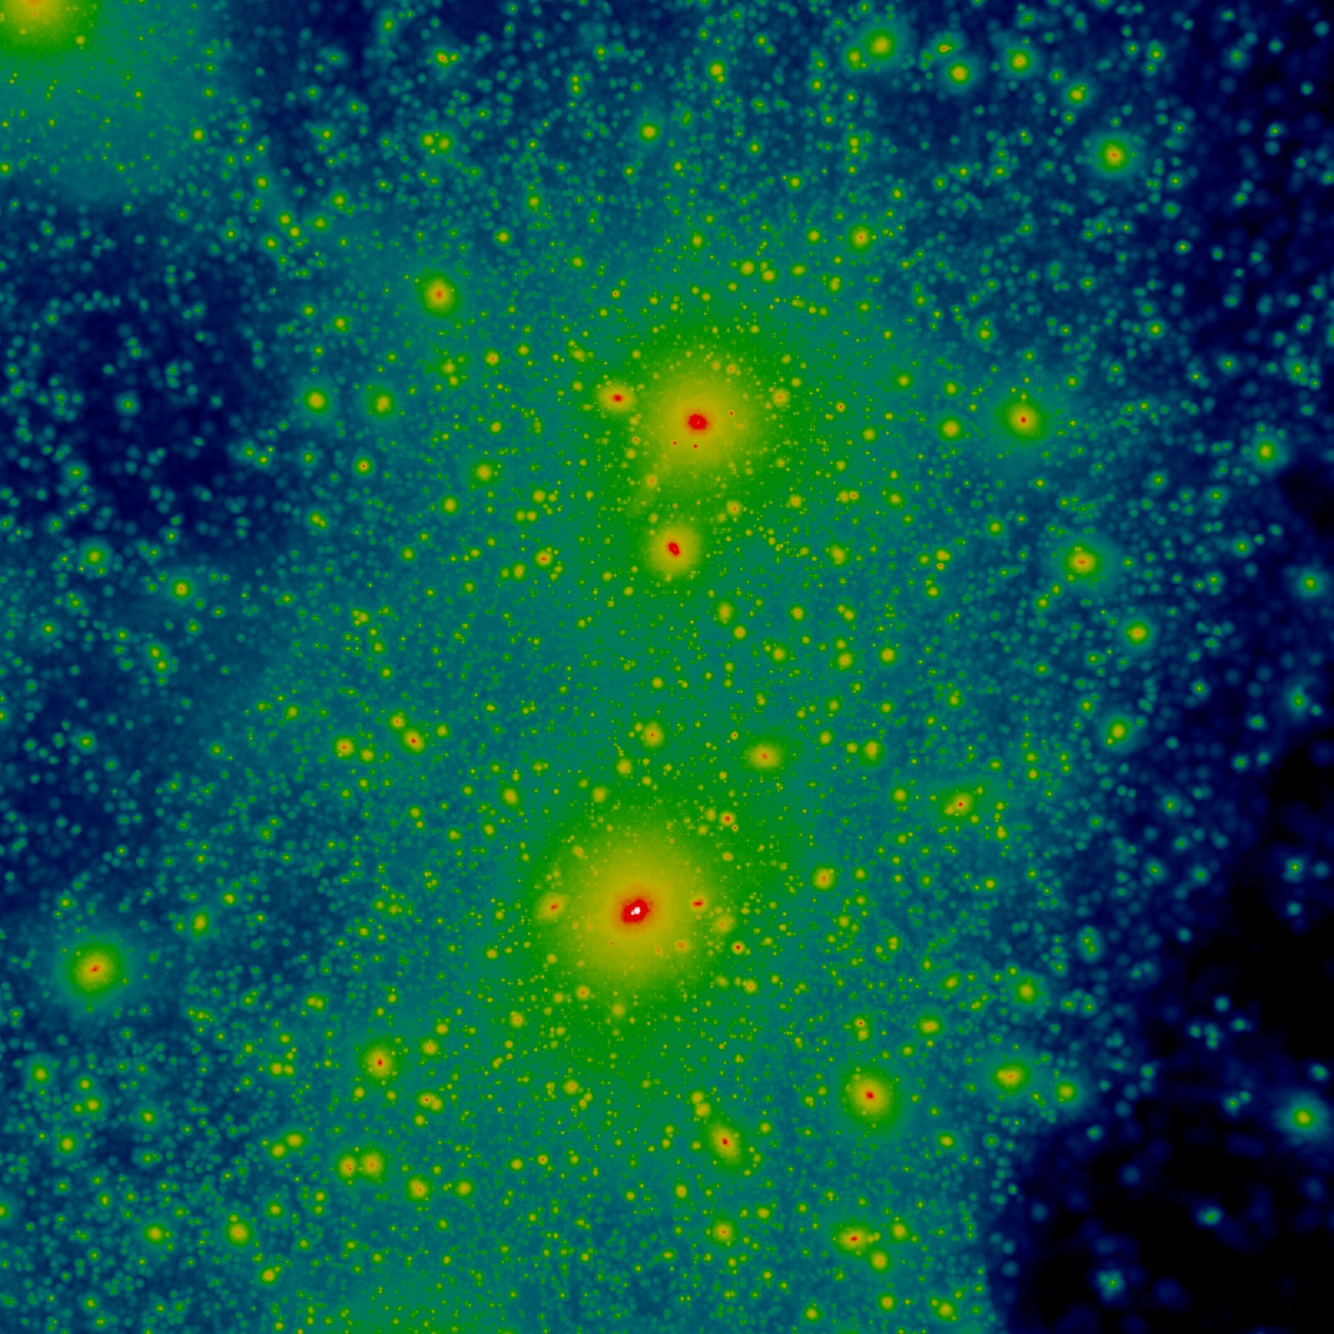
\includegraphics[width=0.3\textwidth]{density.jpg}
\caption{Campo de densidad de Serena-Venus}
\end{figure}

\part[5]Haga un Makefile que genere todos los outputs descritos anteriormente en el órden adecuado.
\end{parts}


\newpage

\question[30] {\bf Integración con el Método del Rechazo}

En un documento \verb+.Rmd+,
 
\begin{parts}
\part[12] Implemente una función que calcule una integral utilizando el método del rechazo \footnote{ Descrito acá: \url{http://en.wikipedia.org/wiki/Rejection_sampling} }. La función debe generar una representación visual del cálculo de la integral (ver Fig.2). Para qué tipo de integrales funciona su solución? 
\part[8] Evalue la integral de la función $h(x) = [cos(50x) + sin(20x)]^2$ sobre $[0,1]$ utilizando el método creado anteriormente. Compare su desempeño con algún método de la función \verb+integrate+.
\part[10] Evalue la integral de la función $p(y) = \int_2^{\infty} \frac{1}{\pi(1+y^2)}$ utilizando el método creado anteriormente. Compare su desempeño con algún método de la función \verb+integrate+.
\end{parts}

A manera de ayuda, la siguiente figura es una representación gráfica del método del rechazo:

\begin{figure}[H]
\centering
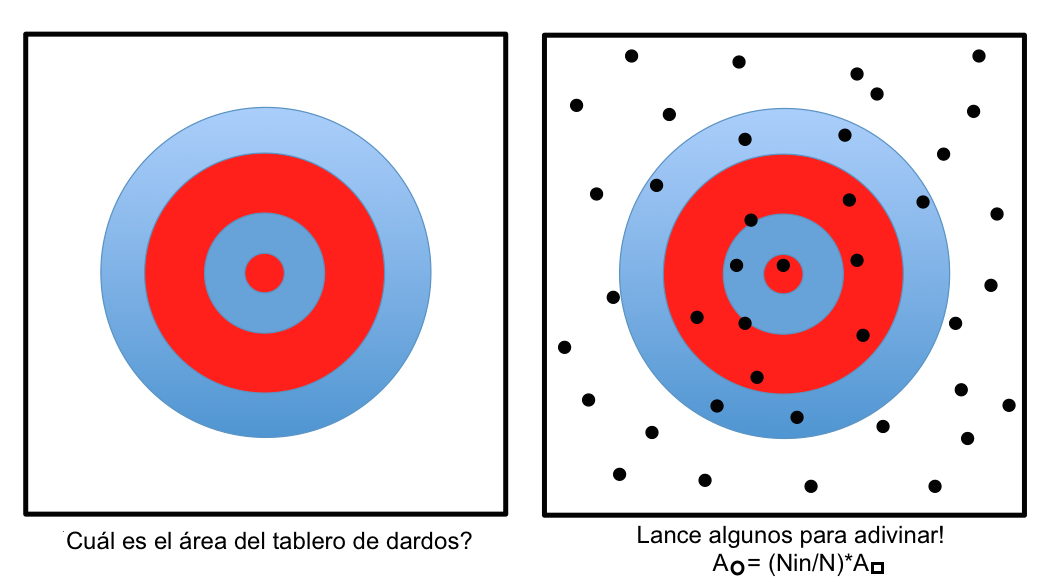
\includegraphics[width=0.8\textwidth]{dardos.png}
\caption{Método de rechazo}
\end{figure}


\end{questions}
\end{document}
